% !TEX encoding = UTF-8 Unicode
\documentclass[aodsor,preprint]{imsart}
\usepackage{amsthm,amsmath,amssymb}
\usepackage{graphicx}
\usepackage[authoryear,round]{natbib}
\usepackage[colorlinks,citecolor=blue,urlcolor=blue]{hyperref}
\usepackage[utf8]{inputenc}
\usepackage{listings}
\usepackage{multirow}
\usepackage{xcolor}
\usepackage{subcaption}
\usepackage{titlesec}
\usepackage{placeins}
\usepackage{float}
\usepackage{siunitx}


% Define custom colors
\definecolor{codegreen}{rgb}{0,0.6,0}
\definecolor{codegray}{rgb}{0.5,0.5,0.5}
\definecolor{codepurple}{rgb}{0.58,0,0.82}
\definecolor{backcolour}{rgb}{0.95,0.95,0.92}

\restylefloat{table}


\titleformat{\section}
{\normalfont\bfseries}{\thesection}{1em}{}
\titlespacing*{\section}{0pt}{0.5em}{0.5em}  % Adjust the spacing as needed

\titleformat{\subsection}
{\normalfont}{\thesubsection}{0.5em}{}
\titlespacing*{\subsection}{0pt}{1em}{1em} 

\titleformat{\subsubsection}
{\normalfont}{\thesubsubsection}{0.5em}{}
\titlespacing*{\subsubsection}{0pt}{1em}{1em} 




% Define custom style
\lstdefinestyle{mystyle}{
    backgroundcolor=\color{backcolour},   
    commentstyle=\color{codegreen},
    keywordstyle=\color{blue},
    numberstyle=\tiny\color{codegray},
    stringstyle=\color{codepurple},
    basicstyle=\ttfamily\small,
    breakatwhitespace=false,
    breaklines=true,
    captionpos=b,
    keepspaces=true,
    numbers=left,
    numbersep=5pt,
    showspaces=false,
    showstringspaces=false,
    showtabs=false,
    tabsize=2
}

% Set the custom style for Python code
\lstset{style=mystyle}
%\usepackage{ngerman}


% settings
%\pubyear{2005}
%\volume{0}
%\issue{0}
%\firstpage{1}
%\lastpage{8}
%\arxiv{arXiv:0000.0000}

\numberwithin{equation}{section}
\theoremstyle{plain}
\newtheorem{thm}{Theorem}[section]
\newtheorem{lemma}[thm]{Lemma}
\newtheorem{corollary}[thm]{Corollary}
\newtheorem{remark}[thm]{Remark}
\newtheorem*{remark*}{Remark}

% customize math operators
\newcommand{\E}{{\mathbb E}}


\begin{document}

\begin{frontmatter}
\title{Forecasting stock price movements using classification methods}
\author{Robert Kovacs\corref{cor1}}

\begin{abstract}
This paper presents an alternative approach to financial time series forecasting by comparing the performance of three machine learning models—Support Vector Machine (SVM), Random Forest (RF), and Naive Bayes—against. The study aims to determine whether these models can predict stock prices more effectively than the traditional benchmark, using real-world data from S\&P 500 components and derived financial information. The findings demonstrate that the proposed approaches offer significant predictive power in the stock market.
\end{abstract}


\begin{keyword}
\kwd{Naive-Bayes classification}
\kwd{Random Forest}
\kwd{Support Vector Machine}
\kwd{Stock market}
\end{keyword}

\end{frontmatter}

\section{Introduction} 

Predicting stock market movements is a complex task due to its dynamic nature, continually influenced by various factors such as the political landscape, overall economic performance, and investor sentiment. Despite efforts to analyze and anticipate these variables, uncertainty persists, complicating the task further. Therefore investors typically adopt one of two approaches when considering investment opportunities in stocks. Firstly, they may assess the fundamental value of a stock, taking into account the aforementioned external factors. On the other hand, technical analysis relies on generated statistics and patterns derived from historical price and volume data to inform decision-making processes (\cite{Kara2011}).

Support Vector Machines, Random Forest, and Naive Bayes are widely applied machine learning models for stock price movement forecasting in the literature. SVM has been frequently used due to its ability to handle high-dimensional data and its effectiveness in binary classification tasks, making it well-suited for predicting upward or downward movements in stock prices. For instance, \cite{kim2003} applied SVM for predicting stock price direction and demonstrated improved accuracy over traditional models. Similarly, \cite{huang2005} found that SVM outperformed other models such as Backpropagation Neural Networks in financial forecasting.

Random Forest, known for its ensemble approach, has also been widely adopted for stock market predictions. Studies like \cite{patel2015} employed Random Forest to capture the complex relationships between technical indicators and stock price movements, showing robust performance due to its resistance to overfitting and its ability to handle large datasets. Naive Bayes, though less commonly used in comparison, has been applied in certain cases such as \cite{henrique2023}, where it was leveraged for its simplicity and efficiency in handling probabilistic relationships, providing a baseline for more complex models.

As prediction variables, common technical indicator (TA) variables, as selected by \cite{Kara2011}, \cite{patel2015}, and \cite{henrique2023}, were used. Their discrete representation, as proposed by \cite{patel2015}, was also employed to explain the future stock price movement direction.

In the current study, we benchmark ensemble methods against single classifier models. The ensemble methods mentioned above use a set of individually trained classifiers as base classifiers. In stock price direction prediction literature, both Support Vector Machines and Random Forests have proven to be top performers (\cite{kumar2006}, \cite{patel2015}).

The relationship between the input window parameter of technical indicators, which determines the period considered by each indicator, and the forecast window was explored by \cite{shynkevich2017}. They found that the highest accuracy was achieved when the lengths of these windows were approximately the same.

In the existing literature, it is common to use approximately 10 years of historical data for stock market analysis, as seen in studies such as \cite{shynkevich2017} (2002–2008), \cite{kim2003} (1989–1999), \cite{patel2015} (2003–2012), \cite{Kara2011} (1997–2008), and \cite{ayyildiz2024} (2012–2022). Our study, however, seeks to improve upon this by creating a more robust framework capable of handling periods of recession. To achieve this, we will include 20 years of data, from January 1, 2004, to December 31, 2023.

In this paper, the data is further subsetted as the forecast window is fixed to 5. To create more realistic circumstances, the dataset is reduced by selecting data based on the day of the week. \hyperref[tab:table1]{Table~\ref*{tab:table1}} shows the distribution of the training and test sets.


\section{Data}
This section outlines the research data, the selection of predictor attributes, and the labeling process. The study focuses on the historical prices of 50 randomly selected stocks, all of which are components of the S\&P 500 stock index. The random selection aims to minimize the risk of highly correlated stock prices, which could lead to similar performance across the prediction models. These stocks are used to develop and evaluate models for predicting price movements.

\medskip

\subsection{Raw data} 

The stock prediction system in this study is applied to forecast future price movements of selected companies from the S\&P 500 index. This index consists of 500 large-cap companies listed on the NASDAQ and NYSE exchanges. For this analysis, only companies with trading records dating back to before January 1, 2004, were considered, and five stocks were randomly chosen for further study. Details of these selected stocks are provided in Appendix A. The raw data was sourced from Yahoo Finance \url{https://finance.yahoo.com/}, and for each stock, 2,640 daily data points were constructed. Each data point provides key information about a stock's performance on a particular day. It includes:

\begin{itemize}
    \item \textbf{Date}: The exact day the data corresponds to.
    \item \textbf{Opening price}: The price at which the stock was first bought or sold when the market opened that day.
    \item \textbf{Closing price}: The price at which the stock was last traded when the market closed.
    \item \textbf{High price}: The highest price the stock reached during the day.
    \item \textbf{Low price}: The lowest price the stock fell to that day.
    \item \textbf{Trading volume}: The total number of shares that were bought or sold during the day.
\end{itemize}

The dataset was subsequently split into training and test sets using an 80:20 ratio. The training set covers the period from January 7, 2004, to December 18, 2019, while the test set spans from January 15, 2020, to December 27, 2023. \\

\medskip

\subsection{Technical indicators - Continuous representation}

Key indicators in financial and technical analysis are essential for assessing market trends, price momentum, and buy or sell signals. Ten technical indicators, calculated using the specified formulas detailed in \hyperref[tab:table4]{Table~\ref*{tab:table4}}, serve as input for predictive models. These indicators provide continuous-valued insight into market behavior and price dynamics. To maintain balance and prevent any single indicator from dominating the analysis, all values are normalized to a range of [-1, +1]. Here, we will discuss these indicators based on definitions from \href{https://www.investopedia.com/}{Investopedia}.\\

The Simple Moving Average (SMA) is a widely used technical indicator that calculates the average price of a security over a specific period, providing a smoothed trend line that helps identify price direction. On the other hand, the Weighted Moving Average (WMA) assigns more weight to recent prices, making it more responsive to recent price changes compared to the SMA.\\

Momentum measures the rate of change of a security's price over a specified time period, indicating the strength of price movements. The Stochastic Oscillator is composed of two lines, \%K and \%D, which compare a security's closing price to its price range over a specific period, highlighting potential overbought or oversold conditions.\\

The Relative Strength Index (RSI) is a momentum oscillator that measures the speed and change of price movements, indicating overbought or oversold conditions.\\

The Moving Average Convergence Divergence (MACD) is a trend-following momentum indicator that shows the relationship between two moving averages of a security's price.\\

Larry Williams' \%R is a momentum oscillator that measures the level of a security's close relative to its highest high over a specific period, indicating potential buy or sell signals.\\

The Accumulation/Distribution (A/D) Oscillator is a volume-based indicator that uses volume flow to predict changes in stock price, combining price and volume to assess the strength of a trend.\\

Lastly, the Commodity Channel Index (CCI) is an oscillator used to identify cyclical trends, measuring a security's deviation from its statistical mean.\\

The descriptive statistics, encompassing minimum, maximum, mean, and standard deviation values for the chosen technical indicators, are detailed in \hyperref[tab:table5]{Table~\ref*{tab:table5}}. These indicators will serve as features in the predictive modeling process.

\subsection{Technical indicators - Trend deterministic representation}

New features were calculated, this is called "Trend Deterministic Data Preparation Layer" in the paper of \cite{patel2015}, and it aims to convert continuous technical indicators into discrete binary variables. This layer translates the indicators into '+1' for upward trends and '-1' for downward trends, simplifying the input for predictive models.\\

If the current price is above the 5-day Simple Moving Average (SMA) or Weighted Moving Average (WMA), the trend is considered upward (+1); otherwise, it is considered downward (-1). \\

Stochastic oscillators such as \%K, \%D, and Williams \%R also signal trends based on their movement relative to the previous period. If the oscillator's value is higher than the previous day, it indicates an uptrend, coded as (+1); otherwise, it suggests a downtrend, coded as (-1). \\

The Moving Average Convergence Divergence (MACD), another trend-following indicator, signals an uptrend (+1) when its value at time t increases compared to t-1, and a downtrend (-1) when it decreases. \\

The Relative Strength Index (RSI) indicates an uptrend (+1) if its value drops below 30, and a downtrend (-1) if it exceeds 70. For values between 30 and 70, if the RSI at time t is greater than at time t-1, it signals an uptrend (+1), and vice versa for a downtrend (-1). \\

If the Commodity Channel Index (CCI) exceeds 200, it signals an uptrend (+1). If it falls below -200, it signals a downtrend (-1). For values between 200 and -200, if the CCI at time t is higher than at time t-1, it is considered an uptrend (+1), and vice versa for a downtrend (-1). \\

The Accumulation/Distribution (A/D) oscillator follows the stock trend, indicating an uptrend (+1) if its value at time t is greater than at time t-1, and a downtrend (-1) if it is lower. \\

A positive momentum value signifies an uptrend (+1), while a negative value indicates a downtrend (-1). \\

Using these indicator values, a trend-deterministic input set is generated and provided to the predictive models. The performance of all models in the study is evaluated based on this representation of the input data as well.

\subsection{Data labeling} 

\cite{shynkevich2017} demonstrated that classification methods such as Support Vector Machines, Artificial Neural Networks, and K-nearest Neighbors perform with the highest accuracy when the input window length is approximately equal to the forecast horizon. In their study of 100 stocks, they observed that among models with equal input window lengths and forecast horizons, setting this parameter to 5 days yields higher accuracy compared to shorter windows. Although accuracy slightly increases up to 30 days, the difference is marginal. Therefore, our study focuses on a case where the technical indicator's input parameter is fixed at 5 days, describing the price behavior over the past 5 days, and the forecast horizon of the models is set to 5 days as well. The decision to use a 5-day forecast horizon is further supported by \cite{zhou2020}, whose results indicate minimal difference in model accuracy between 1, 2, and 3-day forecasting horizons when using SVM.

The target variable is defined by the difference between the closing prices over consecutive 5-day periods:

$$
\text{label}(t,s) = 
\begin{cases} 
1 & \text{,if } \frac{\text{C}_{t+s} - \text{C}_t}{\text{C}_t} > 0 \\
0 & \text{,if } \frac{\text{C}_{t+s} - \text{C}_t}{\text{C}_t} \leq 0
\end{cases}
$$

Here, $t$ represents the time index, $s$ is the forecast horizon (set to 5 days in this case), and $label(t,s)$ indicates whether the closing price increases (1) or decreases (0) over the next $s$ days.

After binning the continuous price changes into discrete categories, we observe that the dataset is largely imbalanced, with different stocks exhibiting significantly varying increase-to-decrease ratios, deviating from the ideal 50-50\%. As suggested by \cite{pagliaro2023}, to avoid bias in the analysis and ensure that each bin contains a representative sample of the data, we applied stratified sampling. By using stratified sampling, we ensure that the resulting models are not biased towards one particular class and are better able to predict outcomes for each class. We address the underrepresented group, typically the downtrend, by sampling an equal number of instances from the other group, without replacement.

%TODO: Add reference to imbalanced table
%TODO: Add reference to final sample size

\section{Predictive models}

\subsection{Naive-Bayes Classifier}
\label{sec:Sub}

The Naive-Bayes classifier assumes that attributes are independent given the class label. It predicts the probability of a data point belonging to a specific class using Bayes’ theorem. This theorem calculates the posterior probability, $\mathbb{P}(C|X)$, based on $\mathbb{P}(C)$, $\mathbb{P}(X|C)$, and $\mathbb{P}(X)$.

\begin{equation}
\mathbb{P}(C|X) = \frac{\mathbb{P}(X|C)\mathbb{P}(C)}{\mathbb{P}(X)}
\end{equation}

Here, $\mathbb{P}(C|X)$ is the posterior probability of class $C$ given data $X$, with $\mathbb{P}(C)$ as the class prior. To compute $\mathbb{P}(X|C)$ efficiently, the classifier assumes attribute conditional independence:

\begin{equation}
\mathbb{P}(X|C) = \prod_{k=1}^{n} \mathbb{P}(x_k|C)
\end{equation}

Eq. 3.2 assumes that each attribute \( x_k \)'s probability given class \( C \) (uptrend class) is independent of the others, simplifying the calculation of the overall probability \( \mathbb{P}(X|C) \). This independence allows the classifier to compute the likelihood of observing data \( X \) under class \( C \) by multiplying individual attribute probabilities, which is computationally feasible even for datasets with many attributes.

For continuous attributes, Gaussian distributions are fitted to the data. The classifier predicts the class label of observation $X$ by comparing the posterior probabilities of each class.

To optimize the Naive Bayes classifier, we apply Grid Search with 5-fold cross-validation to tune the \textit{var\_smoothing} parameter, which adds a small variance to prevent instabilities in the Gaussian Naive Bayes model.

The parameter is searched over 100 logarithmically spaced values from $10^0$ to $10^{-9}$.

\subsection{Random Forest}
\label{sec:Sub}

The random forest algorithm, as described by \cite{Hastie2009}, is a robust ensemble learning technique that uses decision trees as its base models. The core concept of ensemble learning is based on the understanding that a single classifier might not generalize well to new data, particularly when the training set contains noise. To tackle this issue, random forest builds a collection of decision trees by training numerous trees on different portions of the dataset. Each tree is trained using a randomly selected subset of the features, which increases diversity and helps prevent overfitting. During the prediction phase, the algorithm combines the outputs of all trees, with the final class being determined by a majority vote among the trees (\hyperref[fig:plotx]{Figure~\ref*{fig:plotx}}).

\begin{figure}[H]
  \centering
  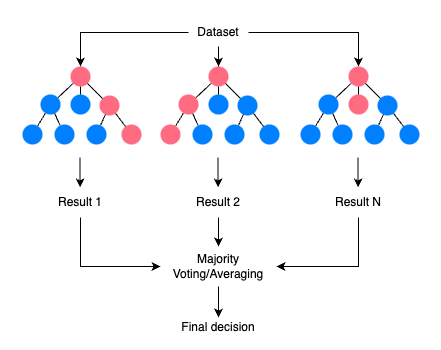
\includegraphics[width=\textwidth]{plots/rf.png}
  \caption{Schematic concept of the Random Forest (\cite{saetia2022})}
  \label{fig:plotx}
\end{figure}


The importance of each feature in the ensemble's decision-making process is visualized in \hyperref[tab:table2]{Table~\ref*{tab:table2}} for the stock Apple Inc. (AAPL), using discrete technical indicators. The model was trained and evaluated on a data set containing only Wednesday trading days for 5-day forecasts. This table ranks features based on their contribution to reducing impurity across all trees in the forest. Higher values indicate more influential features in the model, guiding feature selection and aiding in the interpretation of model predictions.

\begin{table*}[h]
\centering
\caption{Feature Importance Scores for Predictive Model}
\label{tab:table2}
\begingroup
\setlength{\tabcolsep}{10pt}
\renewcommand{\arraystretch}{1.1}%
\begin{tabular}{cc}
    \hline
    \textbf{Feature} & \textbf{Importance} \\
    \hline
    willr   & 0.237624 \\
    macd    & 0.123264 \\
    rsi     & 0.102422 \\
    stochd  & 0.100783 \\
    adosci  & 0.092620 \\
    cci     & 0.090530 \\
    stochk  & 0.077628 \\
    wma     & 0.064612 \\
    sma     & 0.056950 \\
    mom     & 0.053569 \\
    \hline
\end{tabular}
\endgroup
\end{table*}


The number of trees (ntrees) in the ensemble is a crucial hyperparameter that impacts the performance of the model. To efficiently determine the optimal number of trees, as proposed by \cite{patel2015}, the value is varied from 10 to 200 with an increment of 10 each time during the parameter setting procedure, while evaluating performance metrics such as training accuracy and holdout performance. The top-performing configurations, based on these metrics, are then selected for further comparative analysis and model selection. The specific steps involved in the Random Forest algorithm are outlined in \hyperref[tab:table6]{Table~\ref*{tab:table6}}.

For Random Forest models, key hyperparameters include the number of trees in the forest (\textit{n\_estimators}), the maximum number of features considered for splitting a node (\textit{max\_features}), the maximum depth of the tree (\textit{max\_depth}), the minimum number of samples required to split an internal node (\textit{min\_samples\_split}), and whether bootstrap samples are used during tree construction (\textit{bootstrap}). To efficiently determine the optimal values for these parameters, grid search is commonly employed. This technique systematically explores various combinations of hyperparameters to identify the configuration that yields the best performance based on a chosen metric, such as accuracy. Following the approach proposed by \cite{shynkevich2017}, we utilize Grid Search in combination with 5-fold cross-validation. This allows for a thorough evaluation of each hyperparameter combination while ensuring robustness and minimizing overfitting by validating the model's performance across multiple data splits. The possible values of the hyperparameters are summarized in \hyperref[tab:table_rf]{Table~\ref*{tab:table_rf}}.



\begin{table*}[h]
\centering
\caption{Random Forest Hyperparameter Grid}
\label{tab:table_rf}
\begingroup
\setlength{\tabcolsep}{10pt}
\renewcommand{\arraystretch}{2}%
\begin{tabular}{ll}
\hline
\textbf{Hyperparameter} 
& \textbf{Possible Values} \\ \hline
\textit{n\_estimators} 
& $10, 48, 87, 126, 164, 200$ \\
\textit{max\_features} 
& $3$ \\
\textit{max\_depth} 
& $10, 40, 70, 100, \text{None}$ \\
\textit{min\_samples\_split} 
& $2, 4, 8$ \\ \hline
\end{tabular}
\endgroup
\end{table*}

\subsection{Support Vector Machines}
\label{sec:Sub}

Support Vector Machines (SVMs) are powerful algorithms used for classification tasks by employing linear models in high-dimensional feature spaces to accommodate nonlinear decision boundaries. As \hyperref[fig:plotsvm]{Figure~\ref*{fig:plotsvm}} illustrates, SVMs seek to find the maximum margin hyperplane, which optimally separates different classes in the data \cite{kim2003}. This is achieved by mapping input vectors $\mathbf{x}$ into a higher-dimensional space through a nonlinear mapping, represented by a kernel function $K(\mathbf{x}_i, \mathbf{x})$. In the transformed space, SVM constructs a linear model to define the decision boundary. The optimal separating hyperplane is determined by finding support vectors, which are the training examples closest to the hyperplane. The key parameters in SVM, such as the weights $\mathbf{w}$, bias $b$, and coefficients $\alpha$, are computed by solving a constrained quadratic programming (QP) problem, ensuring that the margin between classes is maximized.

\begin{figure}[H]
  \centering
  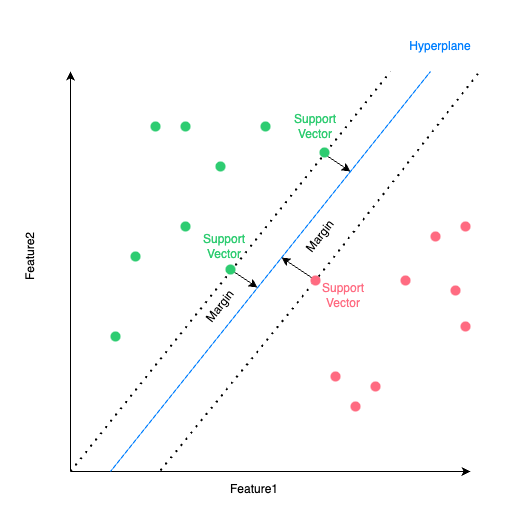
\includegraphics[width=\textwidth]{plots/svm.png}
  \caption{Schematic concept of Support Vector Machines (\cite{james2023})}
  \label{fig:plotsvm}
\end{figure}

As \cite{huang2005} pointed it out, the choice of kernel function significantly influences the model's performance and ability to capture complex patterns in the data. Popular kernels include polynomial kernels $$K(\mathbf{x}_i, \mathbf{x}_j) = (\mathbf{x}_i^\top \mathbf{x}_j + 1)^d$$ and Gaussian radial basis function (RBF) kernels $$K(\mathbf{x}_i, \mathbf{x}_j) = \exp\left(-\frac{1}{2\sigma^2} \| \mathbf{x}_i - \mathbf{x}_j \|^2 \right)$$. These kernels enable SVMs to handle nonlinear relationships by implicitly transforming the data into higher-dimensional spaces where linear separation is feasible. Furthermore, SVMs provide a mechanism to balance the trade-off between maximizing the margin and minimizing misclassification errors through a regularization parameter $C$. By carefully selecting kernel functions and tuning parameters like $d$ (degree of polynomial) and $\sigma$ (bandwidth of RBF), SVMs can be tailored to achieve optimal performance for diverse classification tasks.

The choice of the kernel function, the degree of the polynomial kernel ($d$) when using a polynomial kernel, the gamma parameter ($\gamma$) when using a radial basis function (RBF) kernel, and the regularization constant ($C$) are key parameters of the model.

Similarly to the setup for NB and RF, we apply grid search with 5-fold cross-validation on the training set. Once the optimal parameter values are determined, the predictive capabilities of the SVM models can be compared. This comparison involves utilizing the entire training dataset, applying the optimal parameter values obtained during the parameter tuning phase. Consequently, the models must be re-trained on a new dataset, distinct from the training subset used for parameter tuning, and notably larger. After re-training, the models undergo out-of-sample evaluation using a separate holdout dataset, comprising the remaining portion of the full dataset.




\section{Results}
\subsection{Evaluation metrics}

The classification models employed in this study are tuned through hyperparameter optimization. Due to the range of parameters optimized, the evaluation is based on average metrics for each classification model type. In addition to the classification model type, factors such as the specific day of the week on which the prediction is made and the type of input features—whether continuous or discrete—also influence model performance. We evaluate model performance using the following metrics calculated on the test set: accuracy, precision, recall, specificity, balanced accuracy, and the F1 score. These metrics provide a comprehensive understanding of how well the classifiers, including models such as Random Forest and Support Vector Machines (SVM), perform in predicting stock price movements \cite{pagliaro2023, patel2015}. Furthermore, for financial data performance, \cite{shynkevich2017} introduced the average return and Sharpe ratio as additional evaluation metrics.

\subsubsection{Accuracy}

Accuracy measures the proportion of correctly classified instances out of the total number of instances. It gives a general view of how well a model performs across both positive and negative classes. The formula for accuracy is:

\[
\text{Accuracy} = \frac{TP + TN}{TP + TN + FP + FN}
\]

where:
\begin{itemize}
    \item \( TP \) = True Positives (correctly predicted positive instances)
    \item \( TN \) = True Negatives (Correctly predicted negative instances)
    \item \( FP \) = False Positives (incorrectly predicted positive instances)
    \item \( FN \) = False Negatives (incorrectly predicted negative instances)
\end{itemize}

Although accuracy is a useful metric, it can be misleading in imbalanced datasets, as it may favor the majority class.

\subsubsection{Precision}

Precision is the ratio of true positive predictions to the total number of predicted positive instances. It is particularly important in cases where minimizing false positives is crucial, such as in stock price movement prediction, where predicting upward trends incorrectly could lead to poor trading decisions. The formula for precision is:

\[
\text{Precision} = \frac{TP}{TP + FP}
\]

High precision indicates that the model rarely predicts positive movements (such as price increases) when they do not occur.

\subsubsection{Recall (Sensitivity)}

Recall, also known as sensitivity, measures the proportion of true positive predictions out of all actual positive instances. It is important in scenarios where it is critical to identify all positive instances, such as detecting upward stock price trends. The formula for recall is:

\[
\text{Recall} = \frac{TP}{TP + FN}
\]

A model with high recall ensures that most true positives are detected, though it may come at the cost of increased false positives.

\subsubsection{Specificity}

Specificity is the counterpart to recall, measuring the proportion of true negatives out of all actual negative instances. It is especially useful when distinguishing false positives is important, ensuring that downward trends are not misclassified. The formula for specificity is:

\[
\text{Specificity} = \frac{TN}{TN + FP}
\]

High specificity means that the model correctly identifies instances where stock prices are not predicted to rise, minimizing false alarms.

\subsubsection{Balanced Accuracy}

Balanced accuracy is the arithmetic mean of recall (sensitivity) and specificity. It is a valuable metric for imbalanced datasets, where accuracy alone may not be a reliable indicator of performance. The formula for balanced accuracy is:

\[
\text{Balanced Accuracy} = \frac{1}{2} \left( \frac{TP}{TP + FN} + \frac{TN}{TN + FP} \right)
\]

By balancing the contributions of both true positives and true negatives, balanced accuracy provides a more nuanced view of the model’s effectiveness in situations where one class dominates.

\subsubsection{F1 Score}

The F1 score is the harmonic mean of precision and recall. It is particularly useful when both false positives and false negatives carry significant costs, such as in financial market predictions. The formula for the F1 score is:

\[
\text{F1 Score} = 2 \times \frac{\text{Precision} \times \text{Recall}}{\text{Precision} + \text{Recall}}
\]

A high F1 score indicates a good balance between precision and recall, making it a critical metric when both aspects are important for decision-making.

\subsubsection{Average Return}

The average return measures the mean percentage change in stock value over a given period. It is calculated as:

\[
\text{Average Return} = \frac{1}{N} \sum_{i=1}^{N} R_i
\]

where $R_i$ represents the return at time $i$ compared to the next 5 days' return, and $N$ is the number of the week in the test set. This metric evaluates the model’s ability to capture profitable trades, with higher values indicating better financial performance.

\subsubsection{Sharpe Ratio}

The Sharpe ratio assesses the risk-adjusted return by comparing the excess return (above the risk-free rate) to the standard deviation of returns. It is defined as:

\[
\text{Sharpe Ratio} = \frac{\bar{R} - R_f}{\sigma_R}
\]

where $\bar{R}$ is the average return, $R_f$ is the risk-free rate, and $\sigma_R$ is the standard deviation of returns. A higher Sharpe ratio indicates a model with better risk-adjusted performance.

\subsection{Experimental Results}

\hyperref[fig:plot3]{Figure~\ref*{fig:plot3}} and \hyperref[fig:plot4]{Figure~\ref*{fig:plot4}} present the average accuracy by day of the week for discrete and continuous variables, respectively. 
Each model group consisted of 500 individual models. For each of the 50 selected stocks, we trained 5 distinct models, each corresponding to a specific day of the week. This resulted in 250 models per group. Furthermore, each of these models was trained and evaluated using both continuous and discrete feature vectors. Then we calculated the average evaluation metrics for each model. 

\begin{figure}[H]
  \centering
  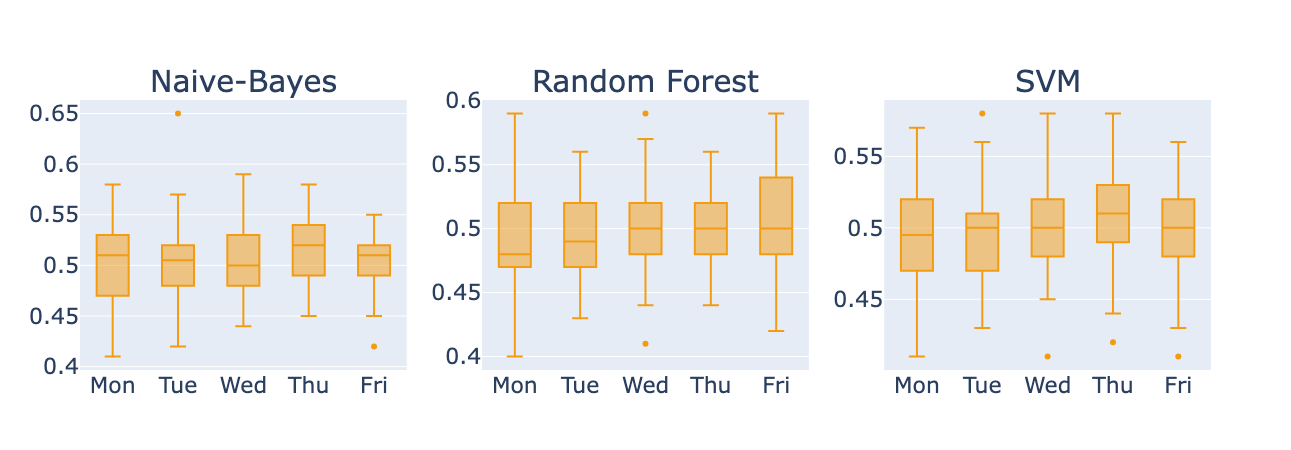
\includegraphics[width=\textwidth]{plots/accuracy_continouos.png}
  \caption{Average Accuracy by Day of Week for Discrete Variables}
  \label{fig:plot3}
\end{figure}

\begin{figure}[H]
  \centering
  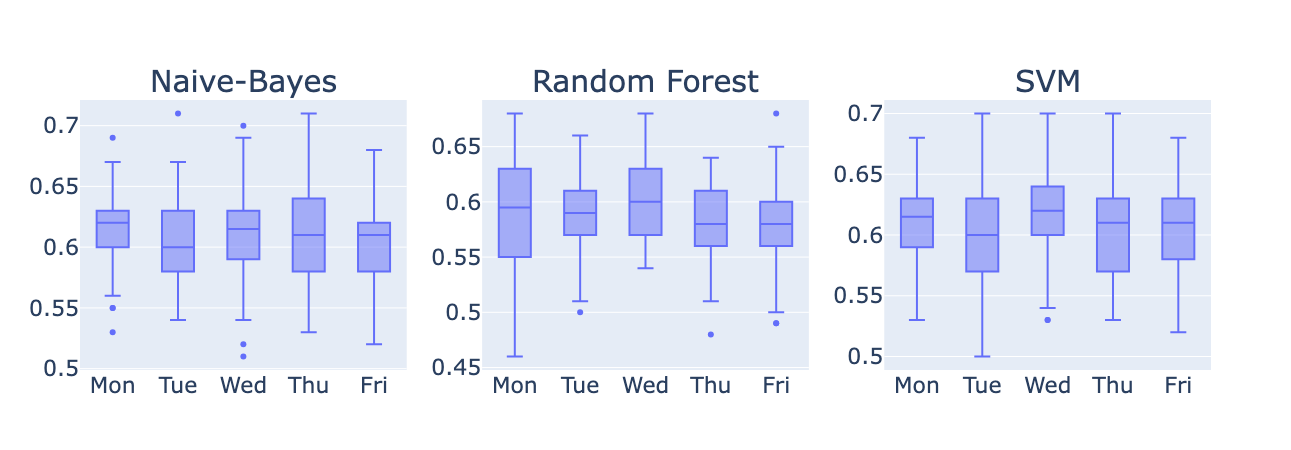
\includegraphics[width=\textwidth]{plots/accuracy_discrete.png}
  \caption{Average Accuracy by Day of Week for Continouos Variables}
  \label{fig:plot4}
\end{figure}

A t-test was employed to determine whether continuous or discrete technical indicators result in higher average accuracy within each model group. Based on the results of the t-tests, there is a statistically significant difference in performance across all three models. For the Naive Bayes classifier, the t-statistic was 31.64, with an extremely small p-value of \num{2.97e-121}, indicating a highly significant difference between the two types of variables. Similarly, the Random Forest model exhibited a t-statistic of 26.48 and a p-value of \num{4.30e-97}, further supporting the presence of a significant difference in accuracy. The SVM model also showed a t-statistic of 32.86 and a p-value of \num{8.42e-127}, confirming a statistically significant difference in accuracy between discrete and continuous variables for this model as well.

Given these extremely low p-values (all well below conventional significance thresholds), we can confidently reject the null hypothesis that there is no difference in average accuracy between discrete and continuous variables for all three models, suggesting that using technical indicators as discrete features can yield higher average accuracy. In the subsequent analysis, we will focus exclusively on the models trained with the discrete representation of the technical indicators.

Comparing the average precision score of the models, it can be observed that the 5-day prediction on Wednesday results in the highest median precision score among all other days, while closer to the weekend, the median precision score for each of the three model groups slightly decreases (\hyperref[fig:plot5]{Figure~\ref*{fig:plot5}}).

Sensitivity across the groups shows a similar range, with the median hovering around 0.6 (\hyperref[fig:plot6]{Figure~\ref*{fig:plot6}}). In the case of Random Forest, all days show similar sensitivity, while for Naive Bayes and SVM, Tuesday has the lowest sensitivity, which increases as the weekend approaches.

Specificity and balanced accuracy exhibit a peak on Wednesday, with relatively smaller variance. However, closer to the weekend, the median of the average specificity drops. Despite this, there is only a slight difference among the models (\hyperref[fig:plot7]{Figure~\ref*{fig:plot7}},\hyperref[fig:plot8]{Figure~\ref*{fig:plot8}}).

Random Forest models tend to have a lower average F-score overall, with the peak occurring on Wednesday and a slight decline towards the weekend (\hyperref[fig:plot9]{Figure~\ref*{fig:plot9}}).

Assessing the average mean return and mean Sharpe ratio across the days of the week and model groups, SVM performs best on Wednesday. Interestingly, although the classification metrics for Random Forest are better than those for Naive Bayes, the profitability metrics favor Naive Bayes over Random Forest in these two categories (\hyperref[fig:plot10]{Figure~\ref*{fig:plot10}}, \hyperref[fig:plot11]{Figure~\ref*{fig:plot11}}).

Finally, as an illustration, SVM models were trained with hyperparameter tuning, as described in an earlier section, for each of the 50 selected stocks over the 4-year test period. A simple strategy was applied using a weekly (5-day) horizon: each week, we buy one unit of a stock if the model predicts an upward trend for the next 5 days, and we sell it on the following Wednesday. Conversely, if the model predicts a downward trend, we short-sell one unit of the stock by borrowing it, selling it at the start of the week, and buying it back one week later to repay the borrowed stock. If the prediction was correct, we gain the change in stock price; otherwise, our portfolio decreases by the percentage of the price change.

The overall performance of the prediction system in this simplified scenario is promising. As shown in \hyperref[fig:svm_performance]{Figure~\ref*{fig:svm_performance}}, with the exception of one underperforming stock, all stocks at least doubled the initial investment, and the best performers increased the initial bankroll by a factor of six over the test period. It is important to note that this scenario does not account for transaction costs or short-selling interest rates, but the results remain encouraging.

\begin{figure}[H]
  \centering
  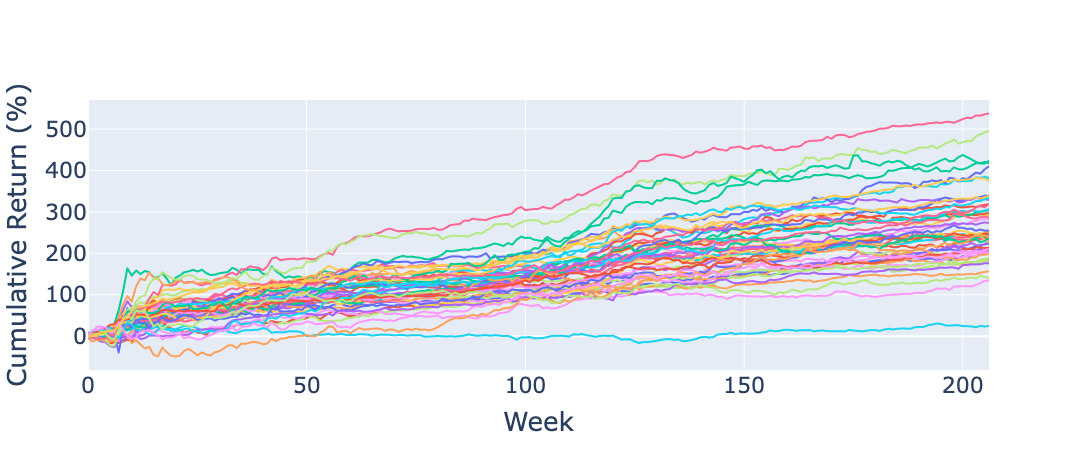
\includegraphics[width=\textwidth]{plots/performance.png}
  \caption{Cumulative return based on SVM prediction}
  \label{fig:svm_performance}
\end{figure}

\section{Discussion}

The comparative analysis of model performances reveals distinctive characteristics and suitability for different forecasting tasks. The examined models — Gaussian Naive Bayes, Random Forest, and Support Vector Machine (SVM) — were evaluated using various classification metrics on the test set, including accuracy, precision, sensitivity, specificity, balanced accuracy, and F1-score. Additionally, we assessed the models' financial performance through metrics like average return and Sharpe ratio to ensure profitability alongside classification power.

Our primary aim in this study was to leverage advanced machine learning techniques to predict significant fluctuations in stock market asset prices. Several technical indicators were employed as inputs to train a set of classifier models. Upon evaluating their performance, we found that our best-performing model was the SVM using a 5-day input window in conjunction with a 5-day forecast horizon, combined with a trend-deterministic layer. This configuration allowed the SVM to capture both short-term and medium-term price movements effectively. 

Interestingly, while the Random Forest model exhibited superior classification power on average across most technical metrics, it was the SVM model that ultimately yielded higher profitability. This discrepancy suggests that although Random Forest can provide more generalized classifications, the SVM excels in accurately predicting significant price changes, particularly in high-volatility scenarios. These findings align with prior work (\cite{kim2003}, \cite{patel2015}), which also observed that SVM models tend to perform better in financial forecasting when it comes to capturing critical price shifts.

However, it is crucial to acknowledge the inherent limitations and complexities involved in stock market predictions. The stock market is a dynamic and nonlinear system influenced by a wide array of factors, many of which are external to the technical indicators typically used in machine learning models. Volatility, macroeconomic events, and unforeseen market shocks can significantly impact prediction accuracy. Thus, while machine learning models like SVM and Random Forest provide valuable guidance, they should not be relied upon for deterministic predictions, and their results should always be interpreted within the broader context of market risks and uncertainties.

To further improve the robustness of machine learning models for stock market predictions, several future research directions can be considered:

\begin{itemize}
    \item \textbf{Expanding Feature Vectors}: SVM models excel when trained on high-dimensional data, as demonstrated in \cite{pagliaro2023}, where the use of more than 20 indicators led to improved forecasting, and \cite{ampomah2020}, which used over 40 technical indicators to enhance prediction accuracy. Expanding the feature set to include a broader range of technical indicators, as well as incorporating non-technical features such as macroeconomic data, can provide a more comprehensive understanding of market dynamics and further enhance model performance.

    
    \item \textbf{Incorporating Fundamental Data}: Stock prices are often influenced by fundamental financial factors related to the performance of companies. As shown in \cite{ballings2015}, the inclusion of fundamental data such as earnings reports and financial ratios can improve prediction outcomes. This suggests that combining technical and fundamental analysis may provide a more comprehensive view of market conditions.
    
    \item \textbf{Integrating Sentiment and External Data}: There is growing evidence that external data sources, such as sentiment and search engine trends, can contribute to more accurate stock market predictions. For example, \cite{saetia2022} integrated Google Trends search data with technical indicators, and \cite{zhou2020} used Baidu search traffic data in their models for Chinese markets. Incorporating similar sentiment data from financial news, social media, or search engine traffic could enhance the predictive power of models, particularly for short-term price movements.
    
    \item Diversifying the Dataset: While our study focused on a specific set of individual stocks, broadening the dataset to include a more diverse portfolio across multiple sectors could help improve the model's ability to generalize across various market conditions. Such an approach would mitigate the risks of sector-specific downturns and improve the robustness of predictions during recessions or economic shifts.
\end{itemize}

\section{Conclusion}

In this paper, we explored the use of machine learning models — SVM, Random Forest, and Gaussian Naive Bayes — for predicting stock price movements using technical indicators. Our findings reveal that SVM outperforms other models in terms of profitability, despite Random Forest showing stronger classification performance. This indicates that SVM may be better suited for predicting significant price fluctuations in volatile markets.

The results highlight the potential of machine learning for stock market prediction, but also emphasize the need for cautious interpretation due to the inherent unpredictability of financial markets. Future research can explore the incorporation of additional feature vectors, fundamental financial data, and sentiment analysis to further improve the predictive capabilities of these models. By expanding the scope of data and refining the models, we can aim to create a more comprehensive and robust framework for stock price movement forecasting.



\newpage

\bibliographystyle{imsart-nameyear}
\bibliography{lit}{}

\newpage


%========= Appendix ==========
\appendix

\section{Selected stock tickers}
\label{sec:appa}

The following 50 randomly selected stocks are analysed: AAPL, AOS, AXP, BA, BAC, BBY, BKNG, CMI, CSCO, CSX, CVX, DIS, DUK, EBAY, ECL, FMC, GE, GIS, GL, HOLX, HUM, IBM, IEX, INTC, IPG, JBHT, JPM, KMB, KO, LUV, MAR, MCD, MNST, NKE, NVDA, OKE, PAYX, PTC, POOL, RL, SBUX, SLB, STE, T, TRV, URI, WAT, WMT, WY



\section{Tables and figures}
\label{sec:appb}

\FloatBarrier

\begin{table*}[h]
\centering
\caption{Train and Test Set Sizes by Day of the Week}
\label{tab:table1}
\begingroup
\setlength{\tabcolsep}{10pt}
\renewcommand{\arraystretch}{1.1}%
\begin{tabular}{cccc}
    \hline
    \textbf{Day} & \textbf{Train Size} & \textbf{Test Size} & \textbf{Total} \\
    \hline
    Monday    & 664  & 188  & 852  \\
    Tuesday   & 674  & 207  & 881  \\
    Wednesday & 680  & 207  & 887  \\
    Thursday  & 658  & 204  & 862  \\
    Friday    & 656  & 202  & 858  \\
    \hline
    \textbf{Total} & \textbf{3332} & \textbf{1008} & \textbf{4340} \\
    \hline
\end{tabular}
\endgroup
\end{table*}


\begin{table*}[h]
\centering
\caption{Selected Technical Indicator Formulas \cite{Kara2011}}
\label{tab:table4}
\begingroup
\setlength{\tabcolsep}{10pt}
\renewcommand{\arraystretch}{2}%
\begin{tabular}{ll} %\begin{tabular}{m{5cm} m{9cm}}
\hline
\textbf{Name of Indicator}
& \textbf{Formula}                                              \\ \hline
Simple $n$-day Moving Average
& $\frac{C_t + C_{t-1} + ... + C_{t-9}}{n}$                     \\ 
Weighted $n$-day Moving Average
& $\frac{(10)C_t + (9)C_{t-1} + ... + C_{t-9}}{n + (n-1) + ... + 1}$
\\ 
Momentum
& $C_t - C_{t-9}$                                               \\ 
Stochastic K\%
& $\frac{C_t - LL_t}{HH_t - LL_t} \times 100$                   \\ 
Stochastic D\%
& $\frac{\sum_{i=0}^{n-1} K_{t-i}}{10}$                         \\ 
Relative Strength Index (RSI)
& $100 - \frac{100}{1 + \left(\sum_{i=0}^{n-1} UP_{t-i}/n\right)/\left(\sum_{i=0}^{n-1} DW_{t-i}/n\right)}$

\\ 
Moving Average Convergence Divergence (MACD) 
& $\frac{MACD(n)_{t-1} + 2}{n+1} \times (DIFF_t - MACD(n)_{t-1})$
\\ 
Larry William’s R\%
& $\frac{H_n - C_t}{H_n - L_n} \times 100$                      \\ 
A/D (Accumulation/Distribution) Oscillator
& $\frac{H_t - C_{t-1}}{H_t - L_t}$                             \\ 
CCI (Commodity Channel Index)
& $\frac{M_t - SM_t}{0.015D_t}$                                 \\ \hline
\end{tabular}
\endgroup
\end{table*}

\begin{table*}[h]
    \centering
    \caption{Random Forest Algorithm}
    \label{tab:table6}
    \begin{tabular}{@{}ll@{}}
    \hline
    \textbf{Step} & \textbf{Description} \\ 
    \hline
    1 & \textbf{Input:} Training set $D$, number of trees in the ensemble $k$ \\
    2 & \quad \textbf{for} $i = 1$ to $k$ \textbf{do} \\
    3 & \quad \quad Create bootstrap sample $D_i$ by sampling $D$ with replacement \\
    4 & \quad \quad Select 3 features randomly \\
    5 & \quad \quad Use $D_i$ and randomly selected three features to derive tree $M_i$ \\
    6 & \quad \textbf{end for} \\
    7 & \textbf{Output:} A composite model $M$ \\
    \hline
    \end{tabular}
\end{table*}


\begin{figure}[H]
  \centering
  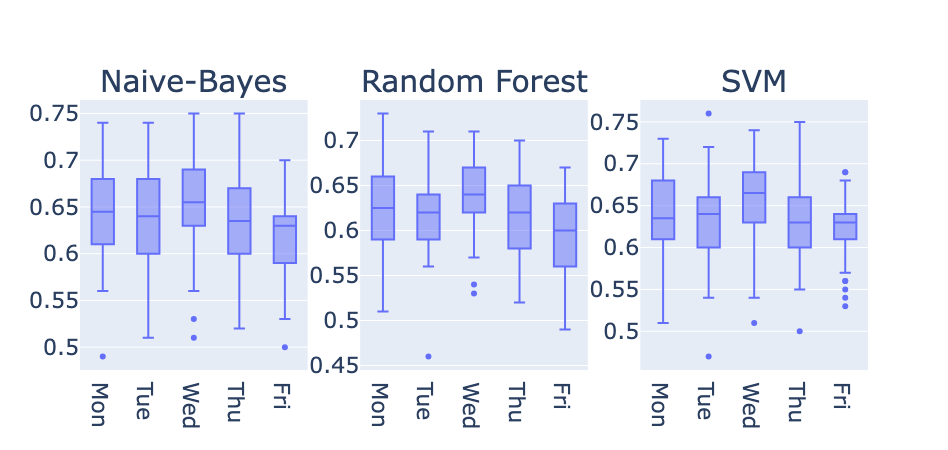
\includegraphics[width=\textwidth]{plots/precision.png}
  \caption{Average Precision by Day of Week for Discrete Variables}
  \label{fig:plot5}
\end{figure}

\begin{figure}[H]
  \centering
  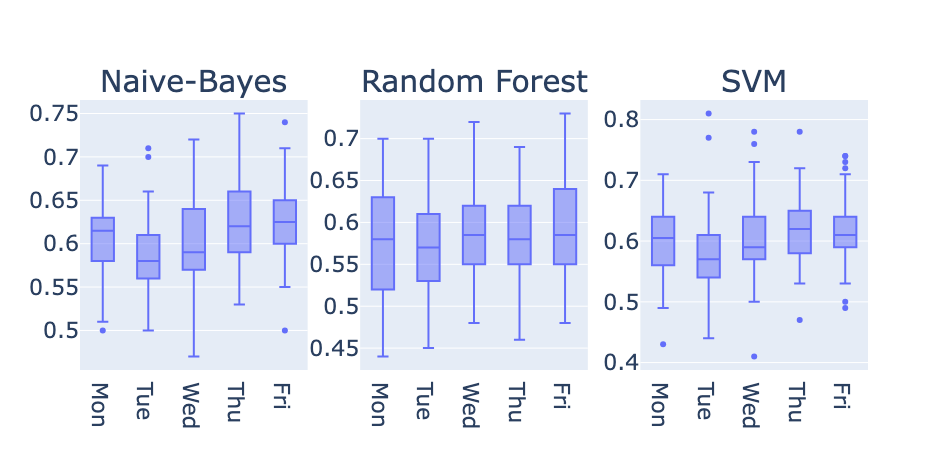
\includegraphics[width=\textwidth]{plots/sensitivity.png}
  \caption{Average Sensitivity by Day of Week for Discrete Variables}
  \label{fig:plot6}
\end{figure}

\begin{figure}[H]
  \centering
  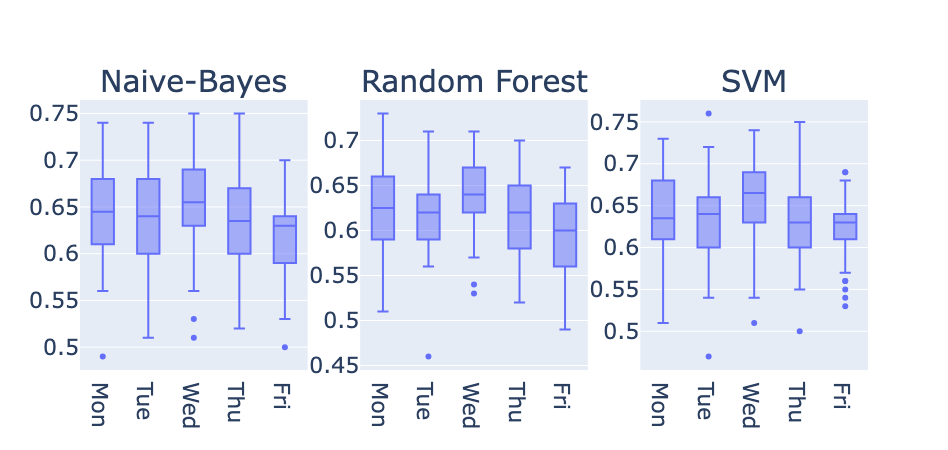
\includegraphics[width=\textwidth]{plots/specificity.png}
  \caption{Average Specificity by Day of Week for Discrete Variables}
  \label{fig:plot7}
\end{figure}

\begin{figure}[H]
  \centering
  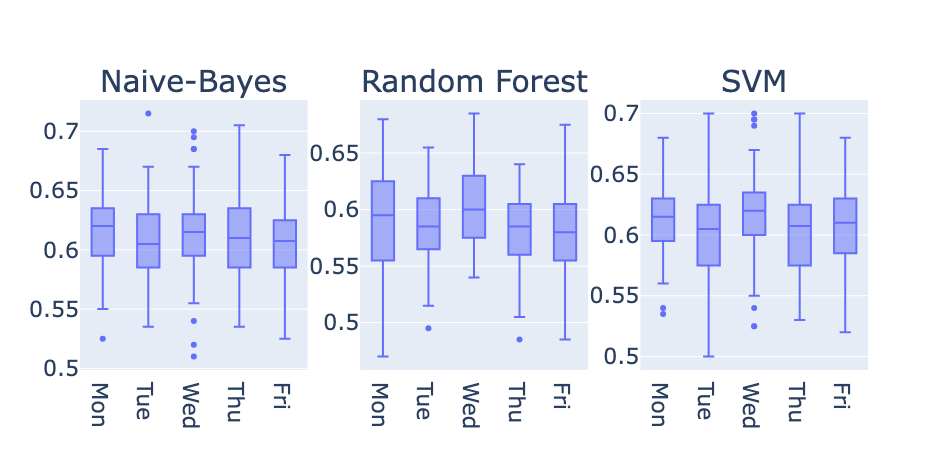
\includegraphics[width=\textwidth]{plots/balanced_accuracy.png}
  \caption{Average Balanced Accuracy by Day of Week for Discrete Variables}
  \label{fig:plot8}
\end{figure}

\begin{figure}[H]
  \centering
  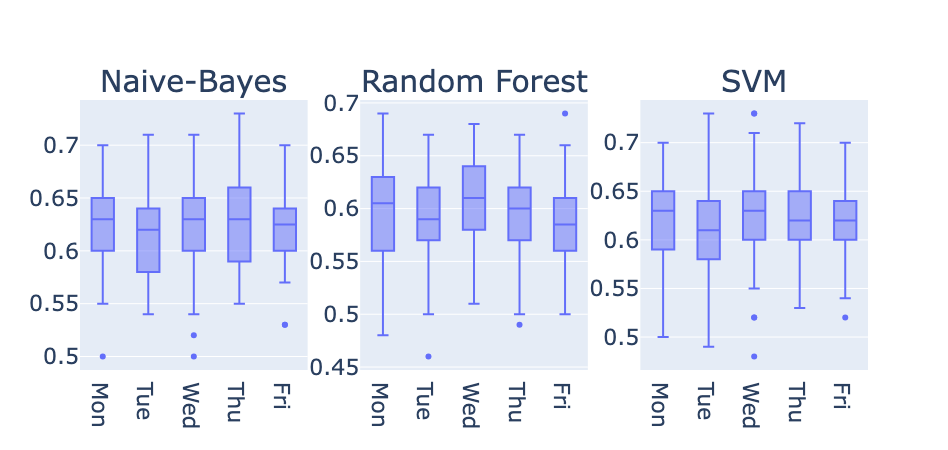
\includegraphics[width=\textwidth]{plots/f-score.png}
  \caption{Average F-score by Day of Week for Discrete Variables}
  \label{fig:plot9}
\end{figure}

\begin{figure}[H]
  \centering
  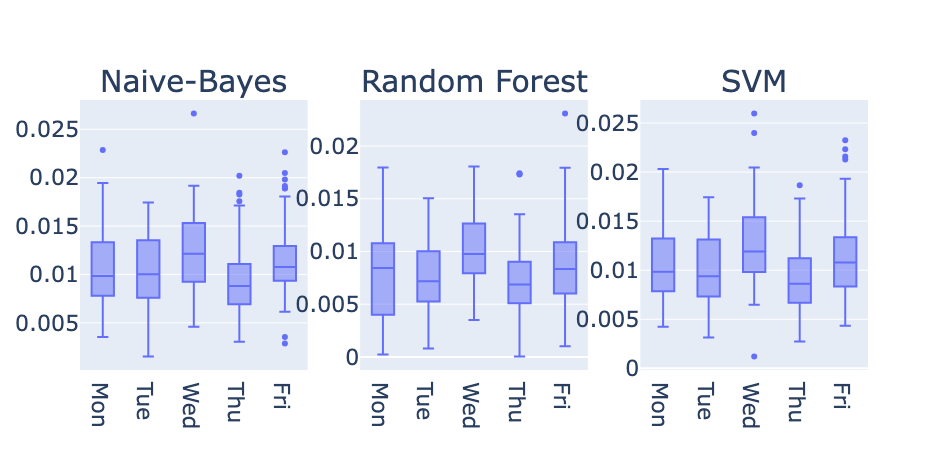
\includegraphics[width=\textwidth]{plots/avg_return.png}
  \caption{Mean of Average Return by Day of Week for Discrete Variables}
  \label{fig:plot10}
\end{figure}

\begin{figure}[H]
  \centering
  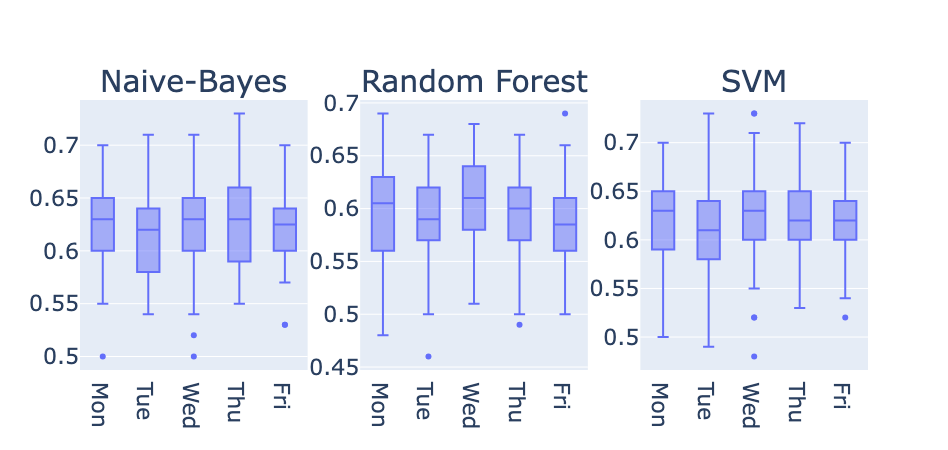
\includegraphics[width=\textwidth]{plots/sharpe.png}
  \caption{Mean of Sharpe Ratio by Day of Week for Discrete Variables}
  \label{fig:plot11}
\end{figure}





\section{Python code}
\label{sec:app}
\begin{lstlisting}[language=Python]

# import the libraries

import pandas as pd
import yfinance as yf
import numpy as np
import talib as ta
import plotly.express as px
from plotly.subplots import make_subplots
from scipy import stats

from sklearn.utils import resample
from sklearn.preprocessing import MinMaxScaler
from sklearn.model_selection import GridSearchCV
from sklearn.naive_bayes import GaussianNB
from sklearn.ensemble import RandomForestClassifier
from sklearn.svm import SVC
from sklearn.metrics import precision_score, recall_score, accuracy_score, f1_score, roc_auc_score


# functions for data preprocessing

def get_data(symbol):
    df = yf.download(symbol, start="1993-01-01", end="2024-01-31")
    df = df.sort_index(ascending=True)
    df.columns = [col.lower() for col in df.columns]
    df = df.drop(columns=['adj close']) 

    return df

def has_missing_values(df):
    return df.isnull().values.any()

# functions for data labeling

def calculate_price_change(df, d):
    df['change'] = df['close'].pct_change(periods=d).shift(-d)
    return df

def calculate_label(df):
    df['label'] = np.where(df['change'] > 0, 1, 0)
    return df

# functions for technical indicator calculation

def calculate_technical_indicators(df, input_window):
    df['sma'] = ta.SMA(df['close'], timeperiod=input_window)
    df['wma'] = ta.WMA(df['close'], timeperiod=input_window)
    df['mom'] = ta.MOM(df['close'], timeperiod=input_window)
    df['stochk'], df['stochd'] = ta.STOCH(df['high'], df['low'], df['close'], fastk_period=14, slowk_period=3, slowd_period=3)
    df['rsi'] = ta.RSI(df['close'], timeperiod=input_window)
    df['macd'], _, _ = ta.MACD(df['close'])
    df['willr'] = ta.WILLR(df['high'], df['low'], df['close'], timeperiod=input_window)
    df['adosci'] = ta.ADOSC(df['high'], df['low'], df['close'], df['volume'], fastperiod=3, slowperiod=10)
    df['cci'] = ta.CCI(df['high'], df['low'], df['close'], timeperiod=input_window)
    return df

def calculate_trend_deterministic(df):
    df['sma'] = np.where(df['close'] > df['sma'], 1, -1)
    df['wma'] = np.where(df['close'] > df['wma'], 1, -1)
    df['mom'] = np.where(df['mom']>0, 1, -1)
    df['stochk'] = np.where(df['stochk'] > df['stochk'].shift(-1), 1, -1)
    df['stochd'] = np.where(df['stochd'] > df['stochd'].shift(-1), 1, -1)
    df['rsi'] = np.where(df['rsi'] > 70, -1, np.where(df['rsi'] < 30, 1, np.where(df['rsi'] < df['rsi'].shift(1), 1, -1)))
    df['macd'] = np.where(df['macd'] < df['macd'].shift(-1), 1, -1)
    df['willr'] = np.where(df['willr'] > df['willr'].shift(-1), 1, -1)
    df['adosci'] = np.where(df['adosci'] > df['adosci'].shift(-1), 1, -1)
    df['cci'] = np.where(df['cci'] > 200, -1, np.where(df['cci'] < -200, 1, np.where(df['cci'] < df['cci'].shift(1), 1, -1)))
    return df

indicators = ['sma', 'wma', 'mom', 'stochk', 'stochd', 'rsi', 'macd', 'willr', 'adosci', 'cci']
    
# indicator scaling

def scale_indicators(df):
    scaler = MinMaxScaler(feature_range=(-1, 1))
    df[indicators] = scaler.fit_transform(df[indicators])
    return df

# functions for sampling

def split_data(df, split_ratio):
    split_index = int(len(df) * split_ratio)
    
    train_df = df.iloc[:split_index]
    test_df = df.iloc[split_index:]
    change_test_df = test_df['change']
    
    return train_df, test_df, change_test_df

def rebalance_data(df):
    train_samples = []

    class_1 = df[df['label'] == 1]
    class_2 = df[df['label'] == 0]

    min_samples = min(len(class_1), len(class_2))

    if min_samples > 0:
        class_1_downsampled = resample(class_1, replace=False, n_samples=min_samples, random_state=42)
        class_2_downsampled = resample(class_2, replace=False, n_samples=min_samples, random_state=42)
        temp = pd.concat([class_1_downsampled, class_2_downsampled])
        train_samples.append(temp)

    train_df = pd.concat(train_samples)
    train_df = train_df.sort_index(ascending=True)

    return train_df

# helper functions for metrics

def print_metrics(y_test, y_pred):
    global metrics_df
    precision_pos = round(precision_score(y_test, y_pred, pos_label=1), 2)
    precision_neg = round(precision_score(y_test, y_pred, pos_label=0), 2)
    recall_pos = round(recall_score(y_test, y_pred, pos_label=1), 2)
    recall_neg = round(recall_score(y_test, y_pred, pos_label=0), 2)
    accuracy = round(accuracy_score(y_test, y_pred), 2)
    f_score = round(f1_score(y_test, y_pred), 2)
    roc = round(roc_auc_score(y_test, y_pred), 2)
    
    metrics = {
        'Precision Positive': precision_pos,
        'Precision Negative': precision_neg,
        'Recall Positive': recall_pos,
        'Recall Negative': recall_neg,
        'Accuracy': accuracy,
        'F-score': f_score,
        'ROC AUC': roc
    }

    for key, value in metrics.items():
        metrics_df.at[metrics_df.index[-1], key] = value

def evaluate_profit(y_test, change_test_df, y_pred):
    df = y_test.copy()
    df = pd.DataFrame(df, columns=['label'])
    df['change'] = change_test_df
    df['prediction'] = y_pred

    df['result'] = np.where(df['prediction'] == df['label'],
                            abs(df['change']),
                            -abs(df['change']))
    
    metrics = {
        'Average Return': df['result'].mean(),
        'Std Return': df['result'].std(),
    }

    for key, value in metrics.items():
        metrics_df.at[metrics_df.index[-1], key] = value
    

# function for fit NB

def fit_nb(X_train, y_train, X_test, y_test, change_test_df):
    param_grid = {
        'var_smoothing': np.logspace(0, -9, num=100)
    }

    gnb = GaussianNB()
    nb_grid = GridSearchCV(estimator=gnb, param_grid=param_grid, verbose=1, cv=5, scoring='accuracy', n_jobs=-1)

    nb_grid.fit(X_train, y_train)

    metrics = {
        'Best Parameters': nb_grid.best_params_,
        'Best Accuracy': nb_grid.best_score_
    }

    for key, value in metrics.items():
        metrics_df.at[metrics_df.index[-1], key] = value

    best_gnb = nb_grid.best_estimator_
    y_pred = best_gnb.predict(X_test)

    print_metrics(y_test, y_pred)
    evaluate_profit(y_test, change_test_df, y_pred)

# function for fit RF

def fit_rf(X_train, y_train, X_test, y_test, change_test_df):
    n_estimators = [int(x) for x in np.linspace(start=10, stop=200, num=6)]
    max_features = [3]
    max_depth = [int(x) for x in np.linspace(10, 100, num=4)]
    max_depth.append(None)
    min_samples_split = [2, 4, 8]
    bootstrap = [True]

    param_grid = {
        'n_estimators': n_estimators,
        'max_features': max_features,
        'max_depth': max_depth,
        'min_samples_split': min_samples_split,
        'bootstrap': bootstrap
    }

    rf = RandomForestClassifier(random_state=42)
    rf_grid = GridSearchCV(estimator=rf, param_grid=param_grid, cv=5, scoring='accuracy', n_jobs=-1)

    rf_grid.fit(X_train, y_train)

    metrics = {
        'Best Parameters': rf_grid.best_params_,
        'Best Accuracy': rf_grid.best_score_
    }

    metrics = {f"{key}": value for key, value in metrics.items()}

    for key, value in metrics.items():
        metrics_df.at[metrics_df.index[-1], key] = value

    best_rf = rf_grid.best_estimator_
    y_pred = best_rf.predict(X_test)

    print_metrics(y_test, y_pred)
    evaluate_profit(y_test, change_test_df, y_pred)

#function for fit svm

def fit_svc(X_train, y_train, X_test, y_test, change_test_df, symbol):
    param_grid = {
        'C': [0.1, 1, 10, 100, 1000],
        'gamma': [1, 0.1, 0.01, 0.001, 0.0001],
        'kernel': ['rbf', 'sigmoid']
    }

    svc = SVC()
    svc_grid = GridSearchCV(svc, param_grid, refit=True, verbose=1, scoring='accuracy', n_jobs=-1, cv =5)

    svc_grid.fit(X_train, y_train)

    best_svc = svc_grid.best_estimator_

    y_pred = best_svc.predict(X_test)

    metrics = {
        'Best Parameters': svc_grid.best_params_,
        'Best Accuracy': svc_grid.best_score_
    }

    metrics = {f"{key}": value for key, value in metrics.items()}

    for key, value in metrics.items():
        metrics_df.at[metrics_df.index[-1], key] = value

    print_metrics(y_test, y_pred)
    evaluate_profit(y_test, change_test_df, y_pred)

# function for creating boxplots

def create_boxplots():
    nb = pd.read_csv("metrics_nb_new.csv")
    rf = pd.read_csv("metrics_rf_new.csv")
    svm = pd.read_csv("metrics_svm_new.csv")

    nb = nb[nb['discrete'] == True]
    rf = rf[rf['discrete'] == True]
    svm = svm[svm['discrete'] == True]


    day_mapping = {0: 'Mon', 1: 'Tue', 2: 'Wed', 3: 'Thu', 4: 'Fri', 5: 'Saturday', 6: 'Sunday'}
    for df in [nb, rf, svm]:
        df['day_of_week'] = df['day_of_week'].map(day_mapping)


    fig = make_subplots(rows=1, cols=3, subplot_titles=("Naive-Bayes", "Random Forest", "SVM"))


    dataframes = [nb, rf, svm]
    titles = ["Naive-Bayes", "Random Forest", "SVM"]


    for i, df in enumerate(dataframes, start=1):
        df['sharp_ratio'] = df['Average Return'] / df['Std Return']


        fig_single = px.box(df, x='day_of_week', y='F-score', title=titles[i-1])
        for trace in fig_single.data:
            fig.add_trace(trace, row=1, col=i)

    fig.update_layout(
        font=dict(size=22),
        showlegend=False
    )

    for annotation in fig['layout']['annotations']:
        annotation['font'] = dict(size=30)

    fig.show()

# function to create ttest

def create_ttest():
    nb = pd.read_csv("metrics_nb_new.csv")
    rf = pd.read_csv("metrics_rf_new.csv")
    svm = pd.read_csv("metrics_svm_new.csv")

    dataframes = {'Naive-Bayes': nb, 'Random Forest': rf, 'SVM': svm}

    for name, df in dataframes.items():
        discrete_group = df[df['discrete'] == True]['Accuracy']
        continuous_group = df[df['discrete'] == False]['Accuracy']
        
        t_stat, p_value = stats.ttest_ind(discrete_group, continuous_group)
        
        t_stat = round(t_stat, 2)
        p_value = p_value
        
        print(f"{name} - T-statistic: {t_stat}, P-value: {p_value}")

# function for creating cumulative return plot

def create_cum_return_plot():
    df = pd.read_csv('svm_predictions.csv')

    symbols = [
        "AJG", "AOS", "BA", "AXP", "BBY", "BKNG", "CMI", "CVX", "CSX", "DIS",
        "DUK", "EBAY", "ECL", "FMC", "GIS", "GL", "HOLX", "HUM", "IBM", "IEX",
        "INTC", "IPG", "JBHT", "JPM", "KMB", "KO", "MAR", "MCD", "MNST", "NKE", 
        "OKE", "PAYX", "POOL", "RL", "SLB", "T", "WAT", "URI", "TRV", "AAPL", 
        "BAC", "CSCO", "NVDA", "WMT", "LUV", "PTC", "SBUX", "WY", "GE", "STE"
    ]


    cum_returns_df = pd.DataFrame()

    for symbol in symbols:
        df[symbol + '_return'] = np.where(df[symbol] == df[symbol + '_label'], 
                                        abs(df[symbol + '_change']*100), 
                                        -abs(df[symbol + '_change']*100))
        df[symbol + '_cum_return'] = df[symbol + '_return'].cumsum()
        cum_returns_df[symbol] = df[symbol + '_cum_return']

    melted_df = cum_returns_df.reset_index().melt(id_vars='index', var_name='Symbol', value_name='Cumulative Return')

    fig = px.line(melted_df, x='index', y='Cumulative Return', color='Symbol', title='Cumulative Returns of Symbols')


    fig.update_layout(
        title=None,
        xaxis_title='Week',
        yaxis_title='Cumulative Return (%)',
        font=dict(size=22),
        showlegend=False
    )

    fig.show()
    
# main loop

columns = ['Precision Positive', 'Precision Negative', 'Recall Positive', 'Recall Negative',
           'Accuracy', 'F-score', 'ROC AUC', 'Best Parameters', 'Best Accuracy', 'Average Return', 'Std Return']
metrics_df = pd.DataFrame(columns=columns)

symbols = [
    "AJG", "AOS", "BA", "AXP", "BBY", "BKNG", "CMI", "CVX", "CSX", "DIS",
    "DUK", "EBAY", "ECL", "FMC", "GIS", "GL", "HOLX", "HUM", "IBM", "IEX",
    "INTC", "IPG", "JBHT", "JPM", "KMB", "KO", "MAR", "MCD", "MNST", "NKE", 
    "OKE", "PAYX", "POOL", "RL", "SLB", "T", "WAT", "URI", "TRV", "AAPL", 
    "BAC", "CSCO", "NVDA", "WMT", "LUV", "PTC", "SBUX", "WY", "GE", "STE"
]


days_of_week = range(5)


for symbol in symbols:
    print(f">>> Processing {symbol}...")
    for day_of_week in days_of_week:
        for is_discrete in [True, False]:

            df = get_data(symbol)

            metrics = {'ticker': symbol, 'day_of_week': 2, 'discrete': True}
    
            if has_missing_values(df) or len(df) < 10:
                metrics['missing'] = 'YES'
                continue
            else:
                pass

            forecast_window, input_window = 5, 5

            df = calculate_price_change(df, forecast_window)
            df = calculate_technical_indicators(df, input_window)

            if not is_discrete:
                df = scale_indicators(df)
            else:
                df = calculate_trend_deterministic(df)

            df = calculate_label(df)
            df = df[(df.index >= '2004-01-01') & (df.index <= '2023-12-31')]

            df = df[df.index.dayofweek == 2]

            train_df, test_df, change_test_df = split_data(df, 0.8)
            train_df = rebalance_data(train_df)

            X_train, X_test = train_df[indicators], test_df[indicators]
            y_train, y_test = train_df['label'], test_df['label']

            metrics['Portion of Positive changes'] = len(y_train[y_train == 1]) / len(y_train)
            metrics['X_train_size'] = len(X_train)
            metrics['X_test_size'] = len(X_test)
            metrics['y_train_size'] = len(y_train)
            metrics['y_test_size'] = len(y_test)

            metrics_df = pd.concat([metrics_df, pd.DataFrame([metrics])], ignore_index=True)

            fit_nb(X_train, y_train, X_test, y_test, change_test_df)
            fit_rf(X_train, y_train, X_test, y_test, change_test_df)
            fit_svc(X_train, y_train, X_test, y_test, change_test_df, symbol)

            pandas_df = pd.read_csv('svm_predictions.csv')
            
            pandas_df[symbol + '_change'] = change_test_df.values
            pandas_df[symbol + '_label'] = y_test.values
            pandas_df.to_csv('svm_predictions.csv', index=False)


metrics_df.to_csv('metrics.csv', index=False)


\end{lstlisting}




\end{document}
